\documentclass{article}
\usepackage{graphicx}
\usepackage{color}
\usepackage{amsmath}
\begin{document}
	\title{GST108-Introduction to Quantitative Reasoning: Managing Money}
	\author{Chikodinaka Daniel Chinaka}
	\maketitle
	\newpage
	\tableofcontents
	\newpage
	\section{Interest Rate}
	\textcolor{red}{Interest(I)} is the price of money. It is the fee paid for borrowing or investing money.\\
	\textcolor{red}{Principal(P)}
is the amount of money being borrowed or deposited.\\
	\textcolor{red}{Interest rate (R)} is the percentage of the principal that uis paid as a fee over a period of time.\\
	\textcolor{red}{Accumulated Balance(A)} is the total amount to be repaid or the total value of money invested.\\
	\textcolor{red}{Simple Interest Formula I=PRT\\
		Accumulated Balance A= P + I\\
		A = P(1+RT)}
	\newpage
	\section{Compound Interest}
	\textcolor{red}{Compound Interest} is interest paid on the original principal of a deposit or loan and also on the accumulated interest.
	The addition of interest to the principal is called \textit{compounding}.
	Interest can be compounded periodically.
	\textcolor{red}{\begin{equation}
			A=P(1+\frac{R}{n})^{nt}
	\end{equation}}
    \textcolor{red}{\begin{equation}
    		I= A+P
    		\end{equation}}
	A = Accumulated Balance or Amount\\
	P = Principal \\ R = Annual Rate (in decimal)\\ n = Number of compounding periods per year\\
	T = Time\\
	I = Interest
	\newpage
	\section{Continuous Compounding}
	Interest accrued on investment of \$1000 at 8\% for 5 years with various compounding periods.\\
	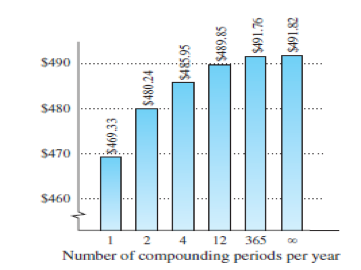
\includegraphics[width=1.0\linewidth]{bar chart.png}
	\newpage
	\subsection{Continuous Compounding}
	Continuous Compounding is when the principal is constantly earning interest and the number of compounding periods increases without bound.
	\textcolor{red}{\begin{equation}
			A=Pe^{RT}
	\end{equation}}\\
	A  =  Accumulated Balance or Amount\\
	P = Principal
\\
	R = Annual Rate (in decimal)
\\
	T = Time
	\newpage
	\section{Effective Rate}
	When interest is compounded, the annual rate of interest (R) is called the nominal rate.\\
	The effective rate, R$_{e}$ is the simple interest rate that would yield the same amount of interest after 1 year.\\
	When a bank advertises a “7\% annual interest rate compounded daily and yielding 7.25\%,” the nominal interest rate is 7\% and the effective rate is 7.25\%. \\
	\textcolor{red}{\begin{equation}
			R_{e} = [(1+\frac{R}{n})^{n-1}]*100
	\end{equation}}\\
	The effective rate is useful for comparing rates with different compounding periods. \\
	\newpage
    \section{Annuity Plan}
	An annuity plan is an investment plan consisting of equal periodic payments.\\
	\textcolor{red}{\begin{equation}
			A = PMT * \frac{[(1+ \frac{R}{n})^{nt} - 1]}{\frac{R}{n}}
		\end{equation}}\\
		A = Accumulated Balance or Amount\\
		PMT  = regular payment  or deposit
\\
		R = Annual Rate (in decimal)
\\
		n = Number of compounding periods per year
\\
		T = Time
\\
			\newpage
		\section{Loan Payment Formula}
		The \textcolor{red}{principal} is the amount of money owed at any particular time. Interest is charged on the loan principal. To pay off a loan, you must gradually pay down the principal\\
		An \textcolor{red}{installment loan (or amortized loan)}is a loan that is paid off with equal regular payments.
\\
		The \textcolor{red}{loan term} is the time you have to pay back the loan in full.
\\
		\textcolor{red}{\begin{equation}
				PMT = \frac{P*\frac{R}{n}}{[1-(1+\frac{R}{n})^{-nt}]}
		\end{equation}}\\
		P = starting loan principal\\
		PMT  = regular payment  or deposit
\\
		R = Annual Rate (in decimal)
\\
		n = Number of compounding periods per year
\\
		T = Time
		\newpage
		\section{Exercises}
		1. Find the simple interest and Accumulated balance for the following:
		\begin{itemize}
			\item Principal = 10000 naira; APR = 8\%; Time = 4 months
			\item Principal = 20000; APR = 6\%; Time = 3 months
			\item Principal = 60,000 naira; APR = 4\%; Time = 2 years
			\item Principal = 50,000 naira; APR = 7\%; Time = 3 years
		\end{itemize}
		
		2. A principal of 20,000 naira earns 6\% per year simple interest. How long will it take for the accumulated balance to become 23000 naira?\\
		3.An account with 10000 naira earns interest at annual rate of  8\%. Find the amount in this account after 10 years if the compounding is  a) monthly    b) daily     c) Quarterly   d) weekly\\
		4.How much money should be deposited in a bank account earning an annual interest rate of 8\% compounded quarterly, in order to have 10 million naira at the end of 10 years?
\\
		5.Every six months, Segun puts 10000 naira into an account earning an APR of 10\% compounded bi-annually. How much will be in the account at the end of 15 years\\
		6.Kunle wants to start a small business in 5 years. He will need 20 million naira to start the business. How much should he deposit every month into an account with an APR of 9\% compounded monthly in order to meet this goal?
		\newpage
		\subsection{Exercises contd.}
		7.Imagine you want to retire in 30 years with a pension of 1,000,000 naira from an investment plan. \\ 
		a)How much money would you have to invest today at an APR of 9\% , compounded daily, in order to have 1,000,000 naira in 30 years? \\
		b)Calculate the total return on investment after 30 years and comment on what will happen to the original investment after 30 years.\\
		c)Calculate the Annual Percentage Yield (APY) on the investment over the 30 year period and comment on what will happen to the original investment every year.\\
		d)How much will the N1, 000, 000 generate in interest each year, if it is invested at an APR of 9\%, compounded daily?
		\newpage
		\subsection{Exercises contd.}
		8.  You want to buy a motorcycle costing 2 million naira. You have two options:
		Option 1 - You can borrow 2 million naira at an APR of 8\% for 1 year and pay it back in monthly payments over the year.\\
		Option 2-   You can save the money you would have made in loan payments during 1 year and purchase the motorcycle.\\
		If you decide to save your money for 1 year:
\\
		a) You will have to deposit the equivalent of 1 month’s loan payment in your savings account at the end of each month, and you will earn 5\% interest on the account, compounded monthly. \\
		b) You will pay 28\% of the interest earned on the savings account in taxes. \\
		c) An annual inflation rate of 7\% will have increased the price of the motorcycle by 7\%.\\
		If you choose the option of saving your money for 1 year, how much money will you have left after you pay the tax and purchase the motorcycle?
		\newpage
		
\includegraphics[width=1.0\linewidth]{bruh.png}
	\end{document}